\documentclass[border=10pt]{standalone}
\usepackage[svgnames]{xcolor}
\usepackage{amsmath}
\usepackage{pgfplots}
\pgfplotsset{compat=newest}
\usepackage[sfdefault]{FiraSans}
\usepackage{FiraMono}
\renewcommand*\familydefault{\sfdefault}
\begin{document}
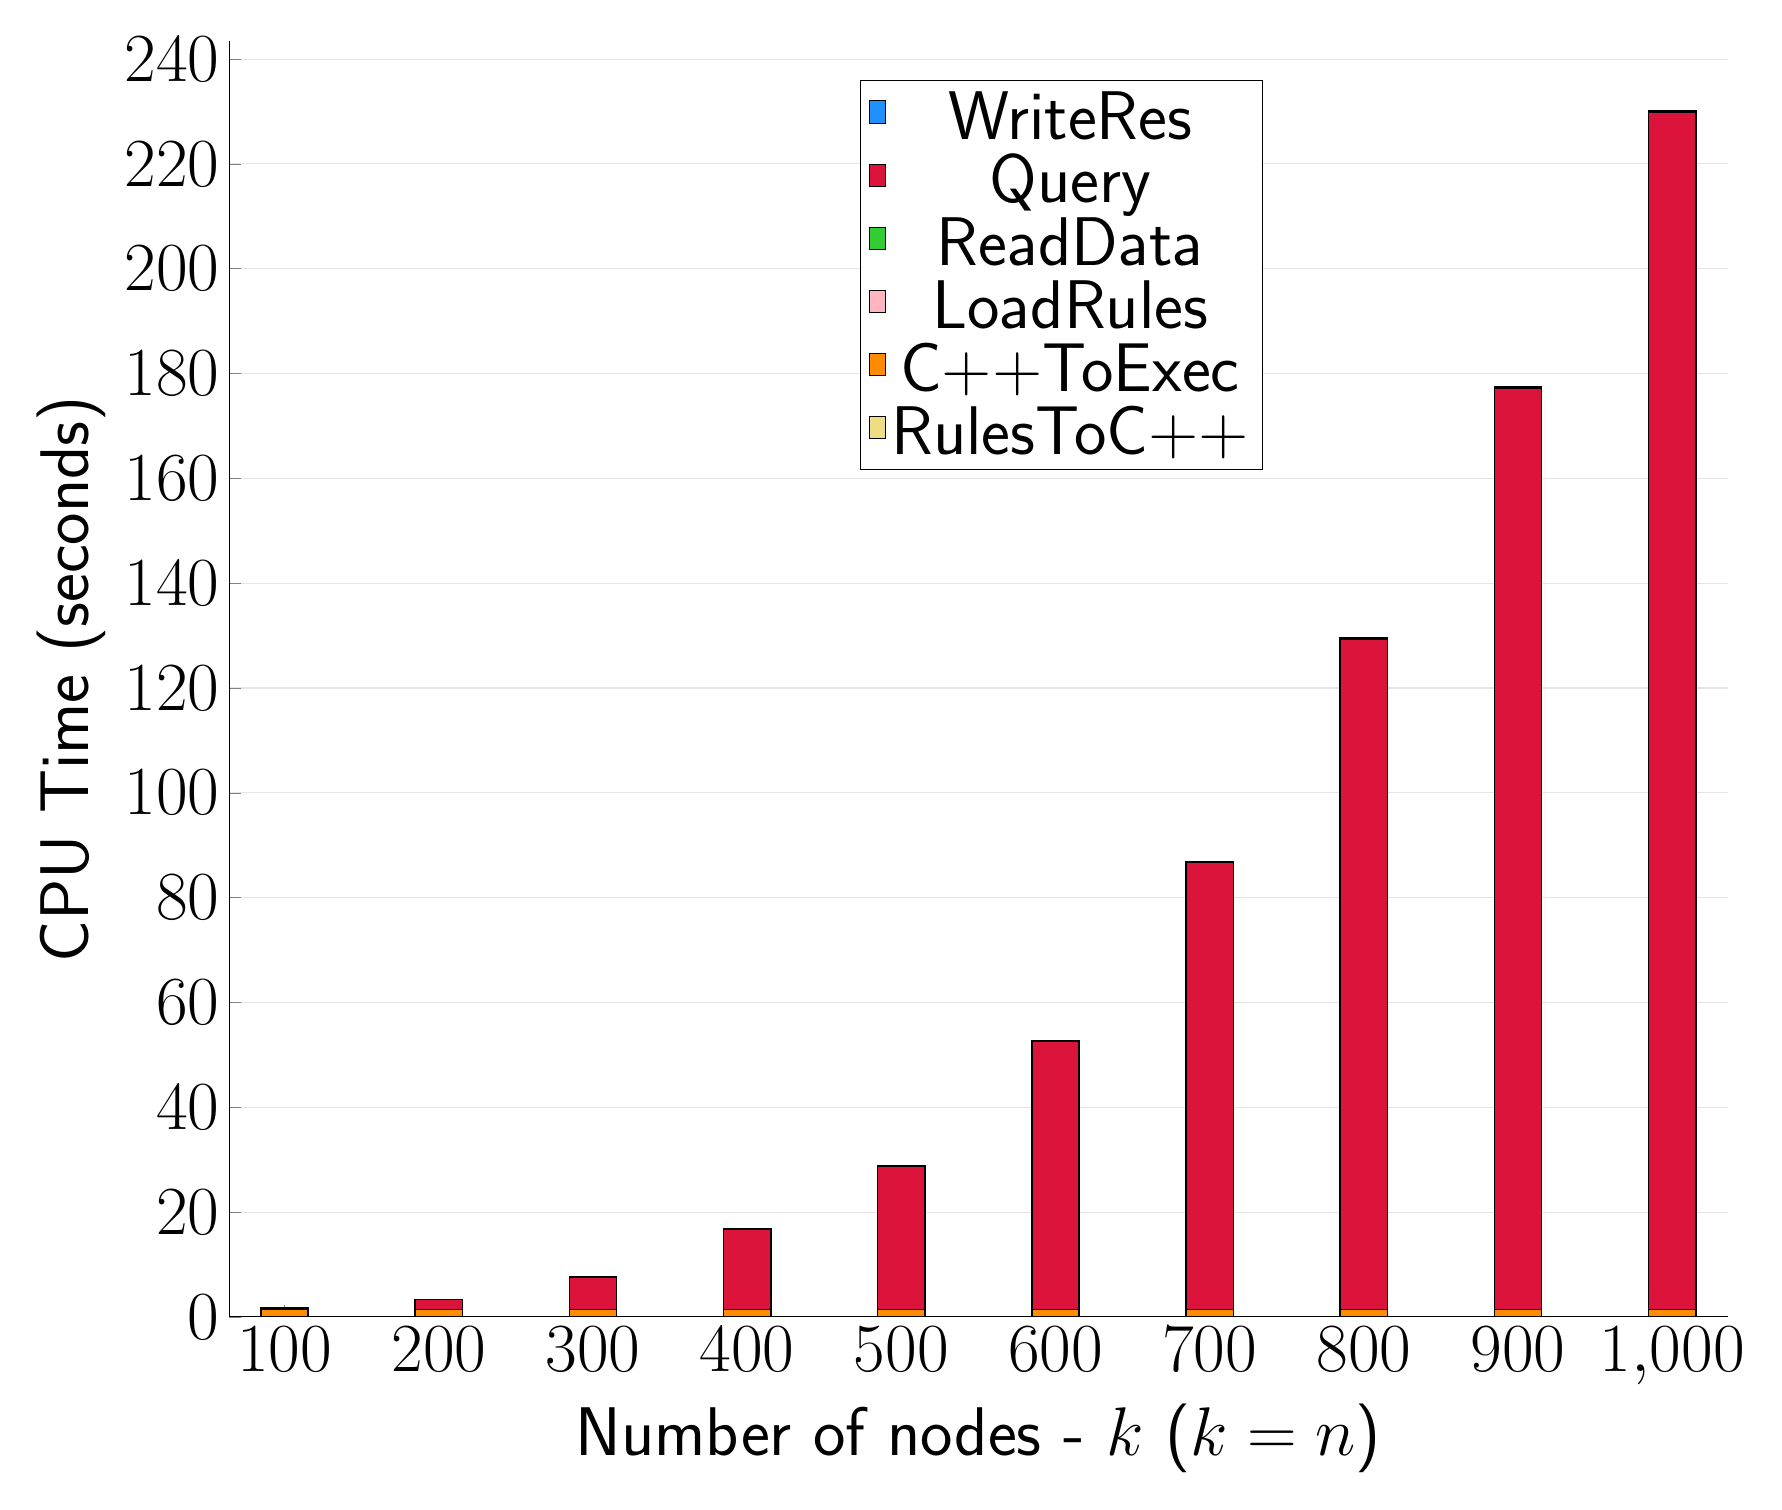
\begin{tikzpicture}
\begin{axis}[
   ybar stacked,
   width=1.7\textwidth,
   bar width=0.6cm,
   ymajorgrids, tick align=inside,
   major grid style={draw=gray!20},
   xtick=data,
   ymin=0, ymax=243.3584,
   axis x line*=bottom,
   axis y line*=left,
   enlarge x limits=0.04,
   legend style={
       at={(0.69, 0.97)},
       anchor=north east,
       legend columns=1,
       font=\Huge,
   },
   ylabel={CPU Time (seconds)},
   xlabel={Number of nodes - $k$ ($k=n$)},
   label style={font=\Huge},
   tick label style={font=\Huge},
]
\addlegendimage{fill=DodgerBlue, draw=black, line width=0.2pt}
\addlegendentry{WriteRes}
\addlegendimage{fill=Crimson, draw=black, line width=0.2pt}
\addlegendentry{Query}
\addlegendimage{fill=LimeGreen, draw=black, line width=0.2pt}
\addlegendentry{ReadData}
\addlegendimage{fill=LightPink, draw=black, line width=0.2pt}
\addlegendentry{LoadRules}
\addlegendimage{fill=DarkOrange, draw=black, line width=0.2pt}
\addlegendentry{C++ToExec}
\addlegendimage{fill=LightGoldenrod, draw=black, line width=0.2pt}
\addlegendentry{RulesToC++}
\addplot +[fill=LightGoldenrod, draw=black, line width=0.55pt] coordinates {
(100, 0.005999999999999997)
(200, 0.004000000000000001)
(300, 0.001999999999999999)
(400, 0.007999999999999997)
(500, 0.0020000000000000018)
(600, 0.004000000000000001)
(700, 0.004000000000000001)
(800, 0.004000000000000001)
(900, 0.006000000000000003)
(1000, 0.00399999999999999)
};
\addplot +[fill=DarkOrange, draw=black, line width=0.55pt] coordinates {
(100, 1.426)
(200, 1.4340000000000002)
(300, 1.4360000000000004)
(400, 1.3980000000000001)
(500, 1.4200000000000002)
(600, 1.4300000000000002)
(700, 1.4180000000000001)
(800, 1.3840000000000001)
(900, 1.3960000000000001)
(1000, 1.4300000000000002)
};
\addplot +[fill=LightPink, draw=black, line width=0.55pt] coordinates {
(100, 0.0001406)
(200, 0.000128)
(300, 0.00015439999999999999)
(400, 2.5e-05)
(500, 0.0001544)
(600, 8.32e-05)
(700, 6.3e-05)
(800, 0.0001492)
(900, 0.0001312)
(1000, 8.999999999999999e-05)
};
\addplot +[fill=LimeGreen, draw=black, line width=0.55pt] coordinates {
(100, 0.0009766)
(200, 0.001098)
(300, 0.0017226)
(400, 0.0015071999999999998)
(500, 0.002681)
(600, 0.0026854)
(700, 0.0024402)
(800, 0.004562999999999999)
(900, 0.004263600000000001)
(1000, 0.0032135999999999996)
};
\addplot +[fill=Crimson, draw=black, line width=0.55pt] coordinates {
(100, 0.23874459999999997)
(200, 1.833512)
(300, 6.199156)
(400, 15.377280000000003)
(500, 27.369139999999998)
(600, 51.1185)
(700, 85.23928)
(800, 127.94380000000001)
(900, 175.8794)
(1000, 228.3584)
};
\addplot +[fill=DodgerBlue, draw=black, line width=0.55pt] coordinates {
(100, 0.0034799999999999996)
(200, 0.0130876)
(300, 0.028773399999999998)
(400, 0.0506958)
(500, 0.0779124)
(600, 0.1127948)
(700, 0.1545674)
(800, 0.2016346)
(900, 0.25612219999999997)
(1000, 0.3147706)
};
\end{axis}
\end{tikzpicture}

\end{document}
